% Created 2023-11-26 dom 17:02
% Intended LaTeX compiler: pdflatex
\documentclass[11pt]{article}
\usepackage[utf8]{inputenc}
\usepackage[T1]{fontenc}
\usepackage{graphicx}
\usepackage{longtable}
\usepackage{wrapfig}
\usepackage{rotating}
\usepackage[normalem]{ulem}
\usepackage{amsmath}
\usepackage{amssymb}
\usepackage{capt-of}
\usepackage{hyperref}
\usepackage{../../modern}
\bibliography{./fuentes.bib}
\raggedbottom
\setcounter{secnumdepth}{2}
\author{Luis Eduardo Galindo Amaya}
\date{sábado, 25 noviembre 2023}
\title{Práctica No. 5 Laboratorio}
\hypersetup{
 pdfauthor={Luis Eduardo Galindo Amaya},
 pdftitle={Práctica No. 5 Laboratorio},
 pdfkeywords={},
 pdfsubject={},
 pdfcreator={Emacs 28.1 (Org mode 9.5.2)}, 
 pdflang={Spanish}}
\begin{document}

\modentitlepage{../../images/escudo-uabc-2022-1-tinta-pos.png}
\datasection{Individual}
\tableofcontents
\pagebreak



\section{Introducción}
\label{sec:org9ccd984}
Durante esta practica utilizaremos sistemas de aprendizaje para
resolver problemas de clasificación y regreción con los problemas
propuestos en el taller anterior se utilizara la bibloteca sklearn y
los ejemplos dados en las clases anteriores. 

\section{Clasificación}
\label{sec:org2acc86e}
\subsection{Problema}
\label{sec:org11032a5}
El problema seleccionado para utilizar clasificación es: Detección de
riesgo de ataque cardiaco. el dataset que se va a utilizar es '\href{https://www.kaggle.com/datasets/rashikrahmanpritom/heart-attack-analysis-prediction-dataset?select=heart.css}{Heart Attack
Analysis \& Prediction Dataset}' de kaggle.

\subsection{Desarollo}
\label{sec:org81ec618}
Para analizar el dataset primero fue necesario cargarlo en el proyecto
para esto se utilizo pandas, una biblioteca del python. Una vez que
tuve el dataset se identificaron las columnas que contenía el archivo:

\begin{center}
\begin{tabularx}{0.8\textwidth}{l|l}
Atributo & Descripción\\
\hline
Age & Edad del paciente\\
Sex & Género del paciente\\
exang & Angina inducida por ejercicio\\
ca & Número de vasos principales\\
cp & Tipo de Dolor de Pecho\\
trtbps & Presión arterial en reposo\\
chol & Colesterol en mg/dl\\
fbs & Azúcar en sangre en ayunas\\
rest\_ecg & Resultados electrocardiográficos en reposo\\
thalach & Frecuencia cardíaca máxima alcanzada\\
target & Riesgo de ataque cardíaco\\
\end{tabularx}

\end{center}

La columna target nos permite identificar que pasientes estan en
riesgo de infarto de manera booleana (verdadero o falso), utilizando
la pagina de \href{https://scikit-learn.org/}{scikit-learn} identifique que algoritmo me podria
clasificar de manera adecuada los datos que tenia y al ser datos de
tipo booleano la regrecion logística.

\subsection{Regresión logística}
\label{sec:org4bbf083}
\autocite{wiki:Logistic_regression} En estadísticas, el modelo
logístico (o modelo logit) es un modelo estadístico que modela la
probabilidad de que ocurra un evento al tener los logaritmos de las
probabilidades (log-odds) para el evento como una combinación lineal
de una o más variables independientes. La regrecion logistica utiliza
como base funcion logistica \autocite{wiki:Logistic_function} la
cual toma un valor y retorna un valor entre 0 y 1:

\[
p(x) = \frac{1}{1 + e^{-( x - \mu )/s}}
\]

donde \(\mu\) es igual al punto medio de la curva y \(s\) es el valor
de escala, la formula entonce se puede reescribir de la manera:

\[
p(x) = \frac{1}{1 + e^{-( \beta_0 + \beta_1 x )}}
\]

donde \(\beta_0 = -\mu / s\) y a este punto se le conoce como la
intercepcion (la intercepcion vertical de \(y\)) y \(\beta_1 = 1/s\).

\begin{figure}[htbp]
\centering
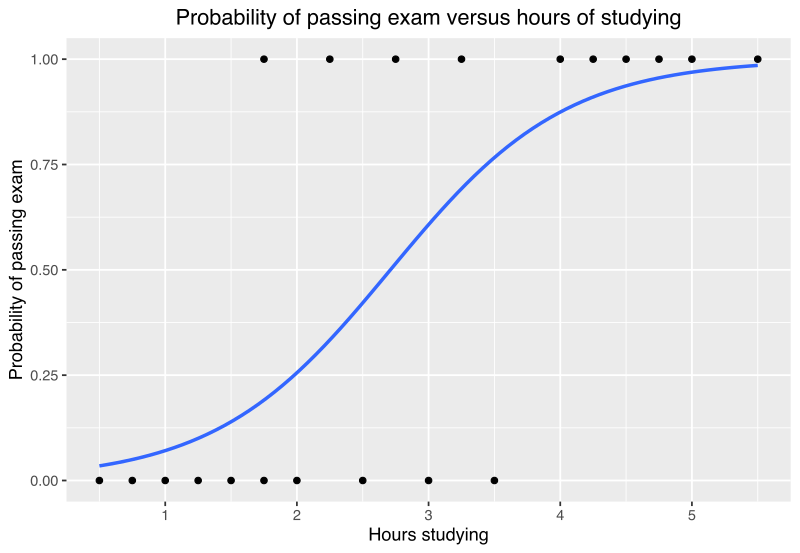
\includegraphics[width=6cm]{img/Exam_pass_logistic_curve.svg.png}
\caption{Ejemplo de regresión logística}
\end{figure}

\subsection{Resultados}
\label{sec:org01d0243}
El modelo da el resultado correcto y es capaz de clasificar
correctamente los valores que se le han enviado, a pesar de que se
movieron algunos parámetros pienso que el algoritmo seleccionado es
óptimo para esta aplicación. 

\begin{figure}[htbp]
\centering
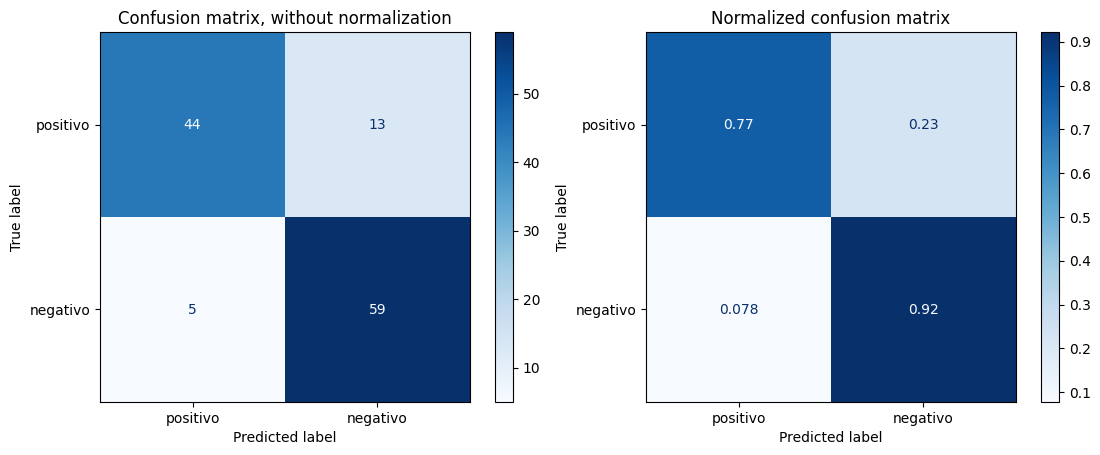
\includegraphics[width=10cm]{img/ddd.png}
\caption{Resultados de la clasificación}
\end{figure}

\section{Regresión}
\label{sec:orgeb22a64}
\subsection{Problema}
\label{sec:orgd88bdfe}
La problematicas seleccionada para el problema de regresion fue la
prediccion de ingresos semanales de una empresa (Walmart), el dataset
que se utilizará es '\href{https://www.kaggle.com/datasets/yasserh/walmart-dataset}{Walmart dataset}'.

\subsection{Desarollo}
\label{sec:org0c7eec7}
Primero se inspeccionaron los datos del dataset, y se pudo identificar
que no todos los datos se pueden usar para la regrecion: 

\begin{center}
\begin{tabularx}{0.8\textwidth}{l|l}
Atributo & Descripción\\
\hline
Store\_Number & Número de la tienda\\
Date & Fecha\\
Week\_of\_Sales & Semana de ventas\\
Weekly\_Sales & Ventas semanales para la tienda dada\\
Holiday\_Flag & Indica si la semana es especial por festividad\\
Temperature & Temperatura el día de la venta\\
Fuel\_Price & Costo del combustible en la región\\
CPI & Índice de precios al consumidor predominante\\
Unemployment & Tasa de desempleo predominante\\
\end{tabularx}

\end{center}

Los datos como el numero de la tienda y la fecha no se pueden usar
para la regreción, las fechas no son solo numeros y los
identificadores no estan ligadas a ningun otro valor que pueda ser
util.

\subsection{Elastic net regularization}
\label{sec:org7bc1120}
\autocite{wiki:Elastic_net_regularization} Para el problema de
regrecion se utilizara el algoritmo ElasticNet, Elastic Net es un
algoritmo de regresión utilizado en estadísticas y aprendizaje
automático. Este algoritmo combina las penalizaciones L1 y L2, que se
utilizan en las técnicas de regresión LASSO (Least Absolute Shrinkage
and Selection Operator) y Ridge, respectivamente. \\


\cite{wiki:LASSO_estadística} Considere una clúster de N casos
(observaciones), cada una con p variable y una sola variable
independente. Sea \(y_i\) la variable independiente y
\(x_i := (x_1,x_2, ... x_p)^T\) el vector con variables para el caso
\(j\). Entonces, el objetivo del Lasso es resolver

\[
\min_{\beta_0, \beta}
\left\{
\frac{1}{N} \sum^N_{i=1}(y_i - \beta_0 -x_i^T \beta)^2
\right\}
\text{sujeto a}
\sum_{j=1}^p | \beta_j | \leq t.
\]

Aquí \(\beta_0\) es el coeficiente constante,
\(\beta:=(\beta_{1}, \beta_{2},..., \beta_{p})\) es el vector de coeficientes
y \(t\) es un parámetro pre especificado que determine la cantidad de
regularizacion. Sea \(X\) la matriz de variables, de manera que
\(\displaystyle X_{ij}=(x_{i})_{j}\) y \(x_{i}^{T}\) es la 'i-esima
fila de \(X\), podemos escribir de forma más compacta el problema
como: 

\[
\min _{\beta _{0},\beta }\left\{{\frac {1}{N}}\left\|y-\beta
_{0}-X\beta \right\|_{2}^{2}\right\}{\text{ sujeto a }}\|\beta
\|_{1}\leq t.
\]


donde \(\|Z\|_{p}=\left(\sum _{i=1}^{N}|Z_{i}|^{p}\right)^{1/p}\)
es la p-norma en dimensiones finitas ( \(\displaystyle \ell ^{p}\) Espacios Lp).

Denotando la media escalar de los puntos \(x_{i}\) como \({\bar {x}}\)
y la media de las variables de salida como \(y_i\) como
\({\bar{y}}\), el estimado para \(\beta_0\) es \({\hat {\beta }}_{0}={\bar
{y}}-{\bar {x}}^{T}\beta\), de modo que:

\[
y_{i}-{\hat {\beta }}_{0}-x_{i}^{T}\beta =y_{i}-({\bar {y}}
-{\bar {x}}^{T}\beta )-x_{i}^{T}\beta
=(y_{i}-{\bar {y}})-(x_{i}-{\bar {x}})^{T}\beta ,
\]

y así es estándar trabajar con variables centralizadas. Adicionalmente
las variables son estandarizadas \(\left(\sum _{i=1}^{N}x_{ij}^{2}=1\right)\)
para que la solución no sea afectada por la escala de las mediciones.

\subsection{Resultados}
\label{sec:org66cd1bc}
El modelo utilizado no es adecuado para la aplicación que se desea por
lo que los resultados obtenidos no pueden predecir los datos de manera
adecuada, se requiere de un mejor entendimiento de los datos para
poder seleccionar una tecnica más adecuada que pueda predecir los
datos obtenidos.

\begin{figure}[htbp]
\centering
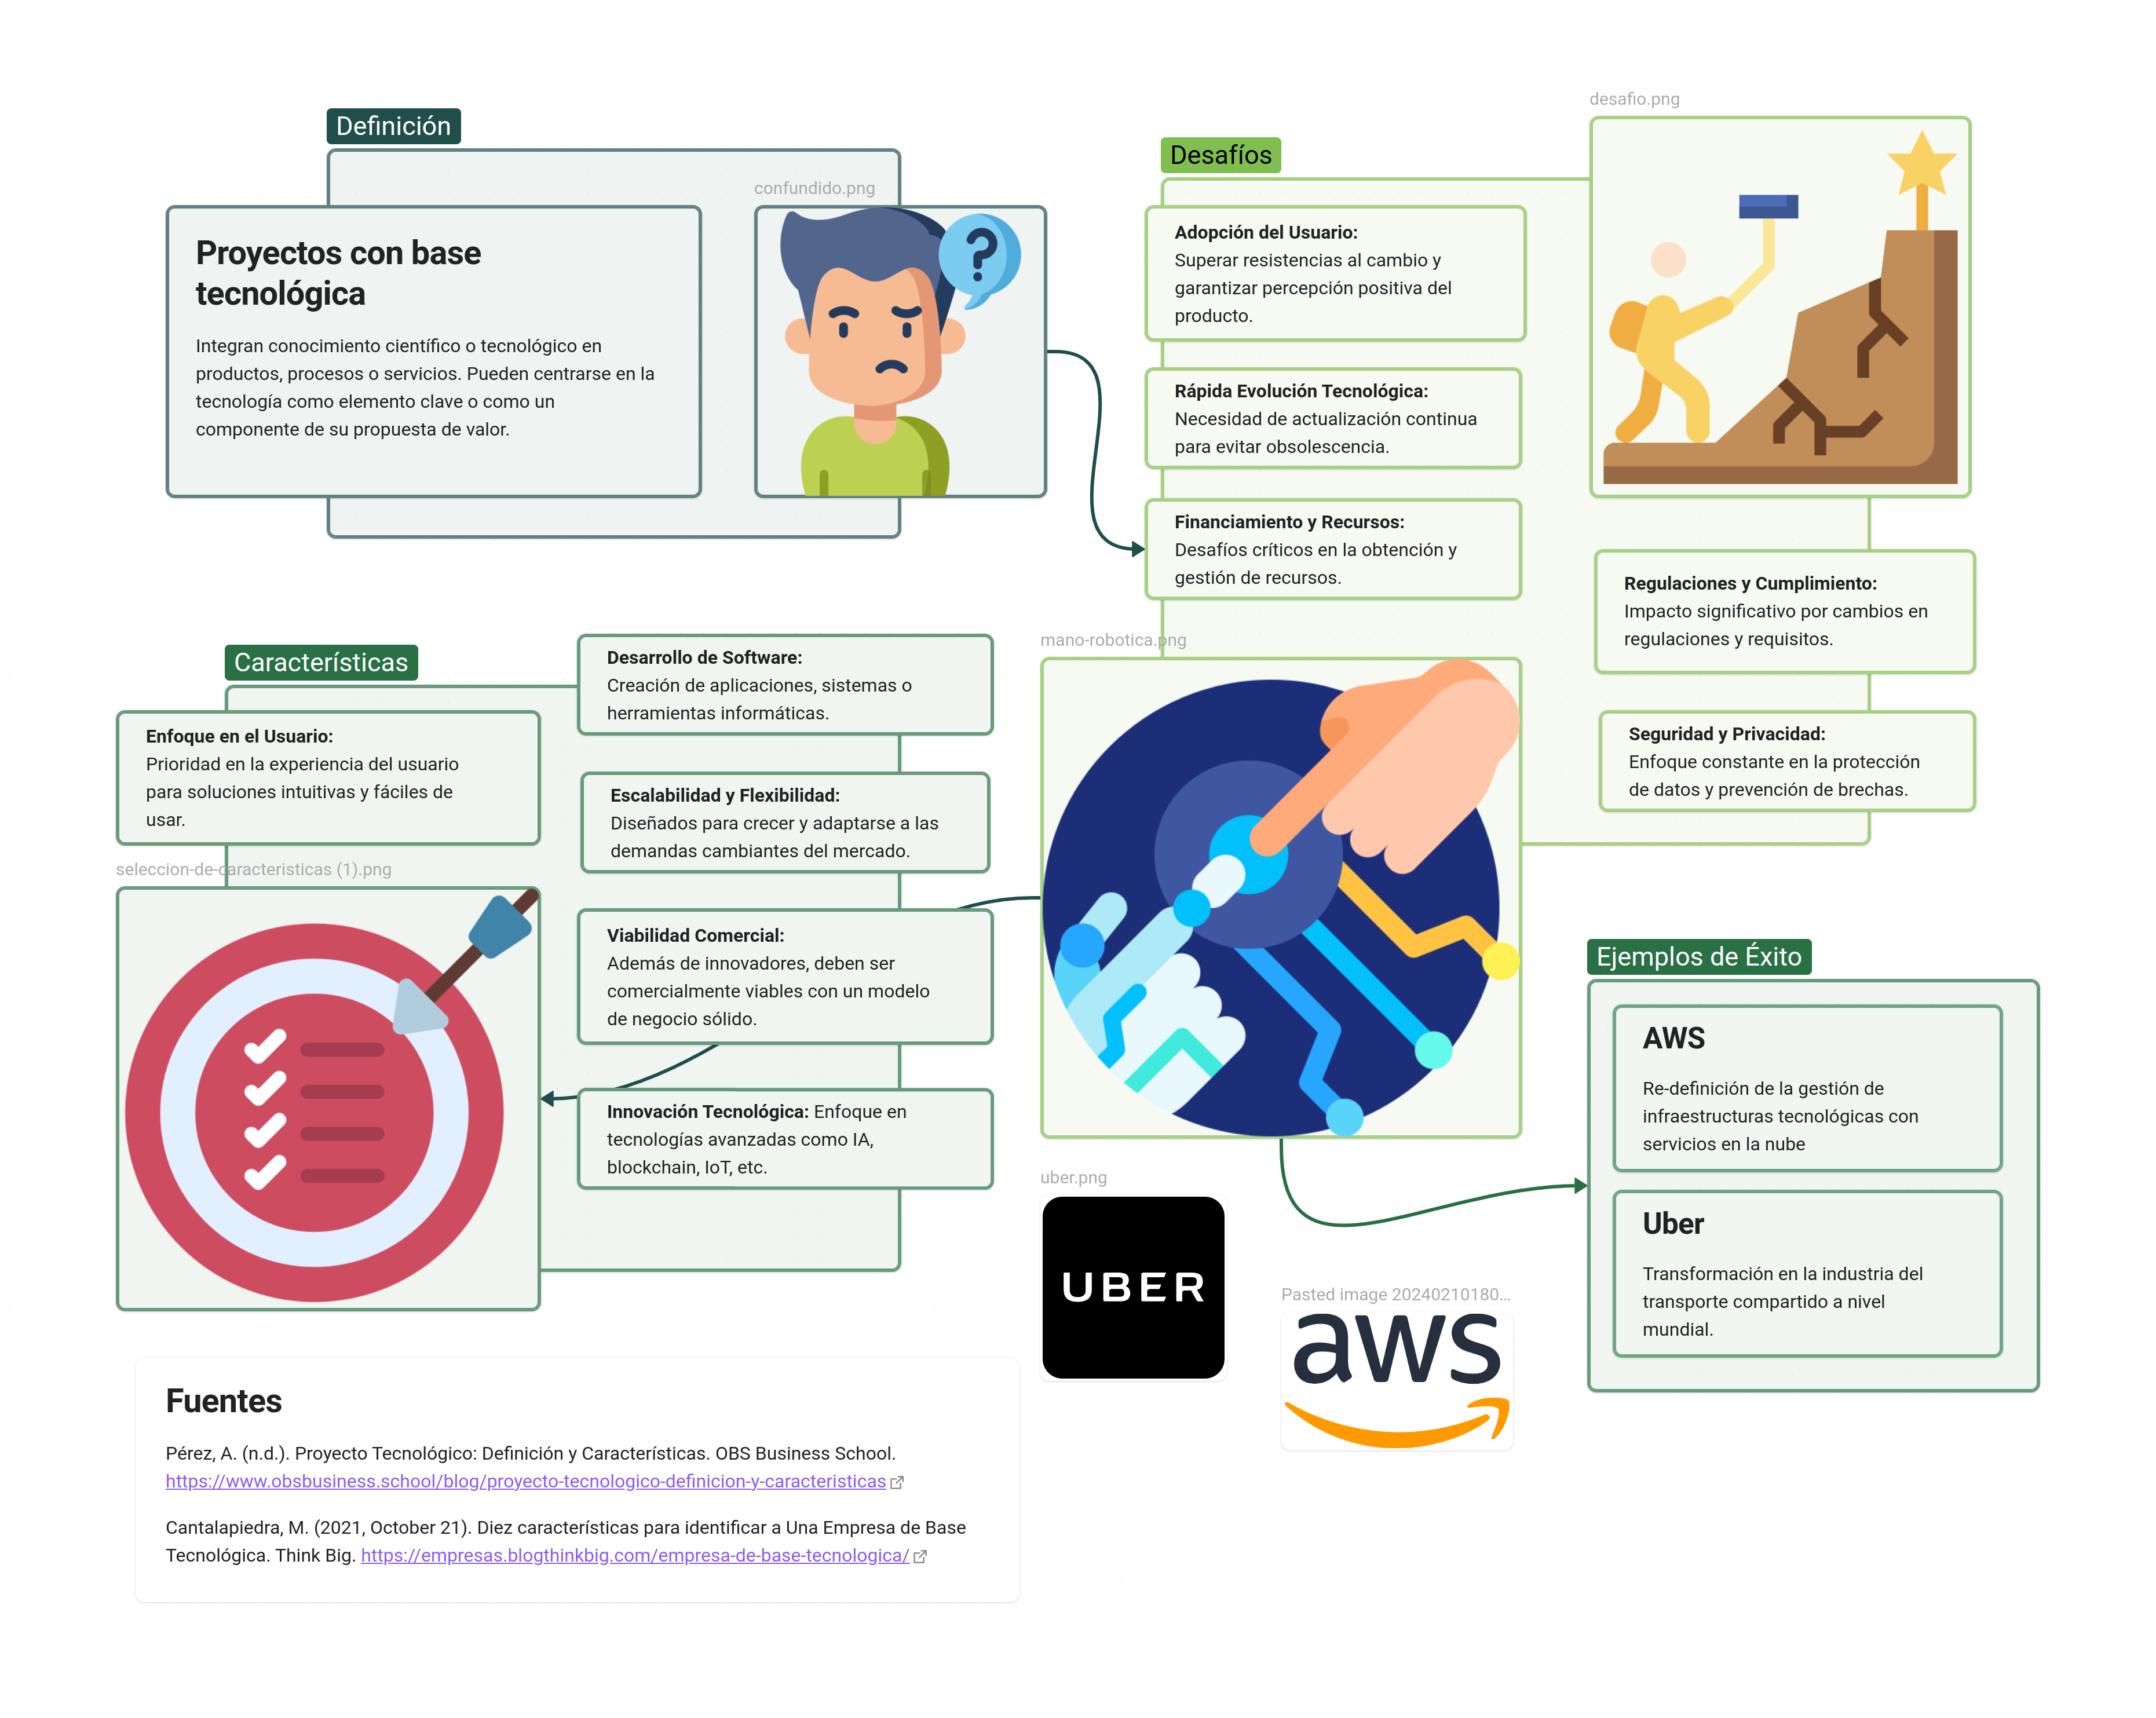
\includegraphics[width=5cm]{img/output.png}
\caption{Los datos predecidos no coinciden con las pruebas}
\end{figure}

\section{Conclusión}
\label{sec:orgce250e4}
Durante esta practica pudimos utilizar herramientas de aprendizaje
para resolver problemas, las herramientas de machine learning permiten
resolver problemas que otras herramientas tendrían más dificultades
explicando. Herramientas como Sklearn permiten usar los algoritmos de
manera fácil sin tener que implementarlos cada vez además que
permiten probar diversas técnicas.


\section{Código}
\label{sec:orgfefbb03}
\subsection{Regresión}
\label{sec:org3da056c}
\begin{verbatim}
 1  from sklearn.model_selection import train_test_split     
 2  import matplotlib.pyplot as plt
 3  import numpy as np
 4  import pandas as pd
 5  from sklearn.pipeline import make_pipeline
 6  from sklearn.preprocessing import StandardScaler
 7  from sklearn.metrics import mean_squared_error
 8  from sklearn.linear_model import ElasticNet
 9  
10  
11  data = [
12      'Store',
13      'Holiday_Flag',
14      'Temperature',
15      'Fuel_Price',
16      'CPI',
17      'Unemployment'
18  ]
19  
20  target = 'Weekly_Sales'
21  
22  dataset = pd.read_csv(
23      "./Walmart.csv",
24      sep=","
25  )
26  
27  X_train, X_test, y_train, y_test = train_test_split(
28       dataset[data], 
29       dataset[target], 
30       test_size=0.4
31  )
32  
33  print(X_train, y_train)
34  
35  model = make_pipeline(
36      StandardScaler(),
37      ElasticNet(
38          alpha=0.1,              # regularizacion del modelo
39          l1_ratio=0.5            # tipo de de penalizacion
40      )
41  )
42  
43  model.fit(X_train, y_train)
44  
45  y_pred = model.predict(X_test)
46  
47  mse = mean_squared_error(y_test, y_pred)
48  print(f"Mean Squared Error: {mse}")
49  
50  sim = model.predict(dataset[data])
51  
52  x = np.linspace(0,sim.size,sim.size)
53  plt.style.use('_mpl-gallery')
54  fig, ax = plt.subplots()
55  ax.scatter(x, sim, s=1, c='blue')
56  ax.scatter(x, dataset[target], s=1, c='red')
57  plt.show()
\end{verbatim}

\subsection{Clasificación}
\label{sec:org5f6f495}
\begin{verbatim}
 1  from sklearn.model_selection import train_test_split     
 2  from sklearn.metrics import ConfusionMatrixDisplay
 3  from sklearn.linear_model import LogisticRegression
 4  import matplotlib.pyplot as plt
 5  import numpy as np
 6  import pandas as pd
 7  
 8  dataset = pd.read_csv(
 9      "./heart.csv", 
10      sep=','
11  )
12  
13  a = dataset[
14      [
15          "age","sex","cp","trtbps","chol","fbs",
16          "restecg","thalachh","exng","oldpeak",
17          "slp","caa","thall"
18      ]
19  ]
20  
21  X_train, X_test, y_train, y_test = train_test_split(
22      a,
23      dataset["output"],
24      test_size=0.4
25  )
26  
27  model = LogisticRegression(
28      penalty="none",             # tipo de penalizacion 
29      c=0.5                       # nivel de regularizacion 
30  ).fit(X_train, y_train)
31  
32  sim = model.predict(X_test)
33  print(y_test)
34  print(sim)
35  
36  titles_options = [
37      ("Confusion matrix, without normalization", None),
38      ("Normalized confusion matrix", "true"),
39  ]
40  
41  for title, normalize in titles_options:
42      disp = ConfusionMatrixDisplay.from_estimator(
43          model,
44          X_test,
45          y_test,
46          display_labels=["positivo", "negativo"],
47          cmap=plt.cm.Blues,
48          normalize=normalize,
49      )
50      disp.ax_.set_title(title)
51  
52      print(title)
53      print(disp.confusion_matrix)
54  
55   plt.show()
\end{verbatim}

\section{Referencias}
\label{sec:org14ddfef}
\printbibliography[heading=none]
\end{document}